\documentclass{article}

\title{ECS 252: Computer Networks \\ Assignment 4}
\author{Yuyang(Peter) Rong \\917781535 \\ PtrRong@ucdavis.edu}

\usepackage[utf8]{inputenc}
\usepackage{graphicx}
\usepackage[colorlinks,linkcolor=red]{hyperref}
\usepackage{amsmath, amsthm, amssymb}
\usepackage[shortlabels]{enumitem}
\usepackage{subfloat}
\usepackage{booktabs}
\usepackage{color}
\definecolor{mygreen}{rgb}{0,0.6,0}
\definecolor{mygray}{rgb}{0.5,0.5,0.5}
\definecolor{mymauve}{rgb}{0.58,0,0.82}

% For listings
% In case we need rust format, check https://github.com/denki/listings-rust
\usepackage{listings}
\lstset{ %
    frame=single,
    % numbers=left,
    backgroundcolor=\color{white},   % choose the background color
    basicstyle=\ttfamily\footnotesize,        % size of fonts used for the code
    breaklines=true,                 % automatic line breaking only at whitespace
    captionpos=b,                    % sets the caption-position to bottom
    commentstyle=\color{mygreen},    % comment style
    escapeinside={(*@}{@*)},         % if you want to add LaTeX within your code
    keywordstyle=\color{blue},       % keyword style
    stringstyle=\color{mymauve},     % string literal style
    tabsize=1,
    % where to put the line-numbers; possible values are (none, left, right)
    numbers = left,
    % how far the line-numbers are from the code
    numbersep = 10 pt,
    % the style that is used for the line-numbers
    numberstyle = \ttfamily,
    % the step between two line-numbers. If it's 1, each line will be numbered 
    stepnumber = 1,
}
\usepackage{ulem}
\usepackage{mathtools}

% For autoref & section reference.
\usepackage{hyperref}
\def\sectionautorefname{Section}
\def\subsectionautorefname{Section}
\def\subsubsectionautorefname{Section}


\usepackage{tikz}
\usepackage{pgfplots}
\usetikzlibrary{shapes,shapes.geometric,backgrounds,arrows,automata,positioning,cd,}
\tikzset{
    cfgedge/.style   = {black, -, >=stealth},
    thickcfgedge/.style   = {black, -, >=stealth, line width=1.1pt},
}
\usepackage{float}

\usepackage{subfigure}

\begin{document}
\maketitle

\section*{Problem 1}

Consider the scenario in which the capacity of the switch fabric is larger than the aggregate capacity of the input ports.
This implies that there is no input queueing.
We consider one of the output ports and model itusing a simple M/M/1 queue.
This implies that we consider that packet arrivals follows a Poisson processwith rate $\lambda$ pkt/sec and the service time to be negative exponential with rate $\mu$ pkts/sec.
We will assume thatthe buffer size (in number of packets) is B.

\begin{enumerate}
      \item Derive an expression for the probability of a packet drop.
      \item We consider the case that the packets are carrying streaming video data using TCP as the transportprotocol.
            We will assume:
            \begin{enumerate}
                  \item segment size is 1500 bytes;
                  \item the round-trip time (RTT) is 200ms;
                  \item the outgoing link data rate is 1 Mbps;
                  \item ignore TCP slow-start.
            \end{enumerate}
            What is the minimum buffer sizerequired to guarantee a QoS of end-to-end throughput of 600 Kbps?
\end{enumerate}

\subsection*{Solution}

\section*{Problem 2}

Consider the network fragment shown in Figure 1
$x$ has two attached neighbours, $w$ and $y$
$w$ has aminimum-cost path to destination $u$ (not shown) of 5 and $y$ has a minimum-cost path to $u$of 6
The completepath from $w$ and $y$ to $u$ (and between $w$ and $y$) are not shown
All link costs in the network have strictlypositive integer values.

\begin{enumerate}
    \item Give $x$ distance vector for destination $w$, $y$, and $u$.
    \item Give a link cost change for either $c(x, w)$ or $c(x, y)$ such that $x$ will inform its neighbor of a newminimum cost path to $u$ as a result of executing the distance-vector algorithm.
    \item Give a link-cost change for either $c(x, w)$ or $c(x, y)$ such that $x$ will not inform its neighbors of a new minimum cost path to $u$ as a result of executing the distance-vector algorithm.
\end{enumerate}

\begin{figure}[H]
    \centering
    \begin{tikzpicture}
        \tikzstyle{every node} = [align=center, draw, circle, node distance = 2cm]
        \node(x){$x$};
        \node[above right of=x](w){$w$};
        \node[above right of=w, draw=none](w1){};
        \node[above of=w, draw=none](w2){};
        \node[right of=x](y){$y$};
        \node[above right of=y, draw=none](y1){};
        \node[right of=y, draw=none](y2){};

        \path (x) edge node[draw=none, above](){1} (w);
        \path (x) edge node[draw=none, below](){4} (y);
        \path (w) edge (w1);
        \path (w) edge (w2);
        \path (y) edge (y1);
        \path (y) edge (y2);
    \end{tikzpicture}
    \caption{Fragment of a network}
\end{figure}

\subsection*{Solution}

\section*{Problem 3}
Consider the network shown in Figure 2 and assume that each node initially knows the cost to each of its neighbors.
Consider the distance vector algorithm and consider the synchronous version that we discussed in class.
Answer the following questions

\begin{enumerate}
      \item Give the initial distance table of all the nodes.
      \item In the first round of exchange of distance vectors many distance vectors will node Z receive?
      \item Determine the distance table of node Z after the first round of exchange of distance vectors among
            the nodes.
\end{enumerate}

\begin{figure}[H]
      \centering
      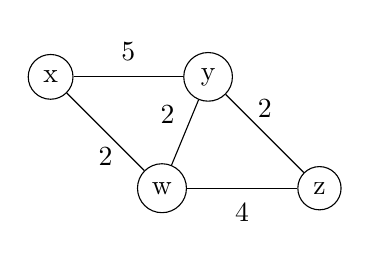
\begin{tikzpicture}
            \tikzstyle{every node} = [align=center, draw, circle, node distance = 2cm]
            \node(x){x};
            \node[right of=x](y){y};
            \node[below right of=x](w){w};
            \node[right of=w](z){z};

            \path (x) edge node[draw=none, below](){2} (w);
            \path (x) edge node[draw=none, above](){5} (y);
            \path (w) edge node[draw=none, above left](){2} (y);
            \path (w) edge node[draw=none, below](){4} (z);
            \path (y) edge node[draw=none, above](){2} (z);
      \end{tikzpicture}
      \caption{A four node network}
\end{figure}

\subsection*{Solution}

\begin{enumerate}
      \item The initial table is shown below:
            \begin{table}[H]
                  \centering
                  \begin{tabular}{lllll}
                        From $x$ & Via $x$ & Via $y$  & Via $z$ & Via $w$  \\
                        To $x$   & -       & -        & -       & -        \\
                        To $y$   & -       & 5        & NA      & $\infty$ \\
                        To $z$   & -       & $\infty$ & NA      & $\infty$ \\
                        To $w$   & -       & $\infty$ & NA      & 2
                  \end{tabular}

                  \vspace{5mm}

                  \begin{tabular}{lllll}
                        From $y$ & Via $x$  & Via $y$ & Via $z$  & Via $w$  \\
                        To $x$   & 5        & -       & $\infty$ & $\infty$ \\
                        To $y$   & -        & -       & -        & -        \\
                        To $z$   & $\infty$ & -       & 2        & $\infty$ \\
                        To $w$   & $\infty$ & -       & $\infty$ & 2
                  \end{tabular}

                  \vspace{5mm}

                  \begin{tabular}{lllll}
                        From $z$ & Via $x$ & Via $y$  & Via $z$ & Via $w$  \\
                        To $x$   & NA      & $\infty$ & -       & $\infty$ \\
                        To $y$   & NA      & 2        & -       & $\infty$ \\
                        To $z$   & -       & -        & -       & -        \\
                        To $w$   & NA      & $\infty$ & -       & 4
                  \end{tabular}

                  \vspace{5mm}

                  \begin{tabular}{lllll}
                        From $w$ & Via $x$  & Via $y$  & Via $z$  & Via $w$ \\
                        To $x$   & 2        & $\infty$ & $\infty$ & -       \\
                        To $y$   & $\infty$ & 2        & $\infty$ & -       \\
                        To $z$   & $\infty$ & $\infty$ & 4        & -       \\
                        To $w$   & -        & -        & -        & -
                  \end{tabular}


                  \caption{
                        ``-'': Connect to self, not applicable cell.
                        ``NA'': not directly connected, i.e. not neighbors.
                        ``$\infty$'': infinity length, as the actual min length is not known yet.
                  }
            \end{table}

      \item Two. Since at the first round $x$ has no idea how to connect to $z$.
      \item The table of $z$ after the first round is:
            \begin{table}
                  \centering
                  \begin{tabular}{lllll}
                        From $z$ & Via $x$ & Via $y$ & Via $z$ & Via $w$ \\
                        To $x$   & NA      & 7       & -       & 6       \\
                        To $y$   & NA      & 2       & -       & 6       \\
                        To $z$   & -       & -       & -       & -       \\
                        To $w$   & NA      & 4       & -       & 4
                  \end{tabular}
                  \caption{
                        ``-'': Connect to self, not applicable cell.
                        ``NA'': not directly connected, i.e. not neighbors.
                        ``$\infty$'': infinity length, as the actual min length is not known yet.
                  }
            \end{table}

\end{enumerate}



\section*{Problem 4}

The following questions are related to the TCP protocol.

\subsection*{Solution}

\begin{enumerate}
    \item \begin{enumerate}
              \item Slow start: 1 ~ 6.
              \item Congestion avoidance: 17 ~ 22.
              \item After 16th: Timeout
              \item After 22nd: Duplicated ACKs
              \item ~32.
              \item ~21.
              \item thessthresh /= 2; window size = thessthresh + 3 MSS.
          \end{enumerate}

    \item It means that you don't need an external clock or other device to sync the operations.
    \item The additive-increase/multiplicative-decrease (AIMD) mean that if there isn't a congestion, the window size is added linearly, i.e. everytime the size is added by an amount.
          If there is one, the size is penalized by a factor.
\end{enumerate}

\section*{Problem 5}

In this problem you will try to derive the efficiency of a CSMA/CD-like multiple access protocol.
We will consider a slotted system in which all the adapters are synchronized to the slot.
The length of the slot (in seconds) is much less than the time to transmit a frame.
Let $S$ be the length of a slot and all frames are of constant length $L=kRS$, where $R$ is the transmission rate of the channel and $k$ is a large integer.
Suppose there are $N$ nodes each with an infinite number of frames to send.
We also assume that $d_{prop} < S$, so that all nodes can detect collision before the end of a slot time.
The protocol is as follows:

\begin{itemize}
      \item If for a given slot, no node has possession of the channel, all nodes contend for the channel; inparticular, each node transmits in the slot with probability $p$.
            If exactly one node transmits in the slot, that node takes possession of the channel for the subsequent $k-1$ slots and transmits its entire frame.
      \item If some node has possession of the channel, all other nodes refrain from transmitting until the node that possesses the channel has finished transmitting its frame.
\end{itemize}

Once this node has transmitted its frame, all node contend for the channel.
Note that the channel alternates between two states: the productive state, which last exactly $k$ slots, and the non-productive state which lasts for a random number of number of slots.
The channel efficiency is the ratio of $k/(k+x)$ where $x$ is the expected number of consecutive unproductive slots.

\begin{enumerate}
      \item For a fixed $N$ and $p$, determine the efficiency of this protocol.
      \item For a fixed $N$, determine $p$ that maximizes the efficiency.
      \item Using the $p$(which is a function of N)found in (b), determine the efficiency as $N$ approaches infinity.
      \item Show that this efficiency approaches 1 as the frame length becomes large.
\end{enumerate}

\subsection*{Solution}

\begin{enumerate}
      \item The probability of successfully get the channel:
            $$P = {N \choose 1}p(1-p)^{N-1}$$
            The probability function of the number of consecutive unproductive:
            $$f(x) = (1-P)^{x-1}P$$
            Thus the expected waiting unproductive slots is:
            $$E(X) = \sum_s^N sf(s) = \frac{P}{1-P}\sum_s^N s(1-P)^s = \frac{P}{1-P}\frac{1-P}{P^2} = 1/P $$
            Thus the efficiency is:
            $$ \frac{k}{k+x} = \frac{k}{k+1/P-1} = \frac{Npk(1-p)^{N-1}}{Np(k-1)(1-p)^{N-1} + 1}$$

      \item To maximize the efficiency, is to minimize $1/P$, i.e. maximize $P$.
            For fixed $N$ we have: $$P(p) = Np(1-p)^{N-1}, p \in (0, 1)$$
            $\log$ is a monotone function, thus taking log wouldn't affect the maximuze point of this function, but taking derivitive would be much easier:
            $$L(p) = \log P(p) = \log N + \log p + (N-1)\log (1-p), p \in (0, 1)$$
            $$L'(p) = \frac{1}{p} - \frac{N-1}{1-p}$$
            The zero point of $L'(p) = 0$ is $p = \frac{1}{N}$.
            Therefore when $p \in (0, \frac{1}{N}], L'(p) > 0, L(p)$ increases, $P(p)$ increases.
            When $p \in [\frac{1}{N}, 1), L'(p) < 0, L(p)$ decreases, $P(p)$ decreases.

            Thus $P(p)$ is maximuzed when $p = \frac{1}{N}$, $P(\frac{1}{N}) = (\frac{N-1}{N})^{N-1}$

      \item Using results in 1) and 2), when $p = \frac{1}{N}$, we have:
            $$\lim_{N \rightarrow \infty} \frac{1}{P} = \lim_{N \rightarrow \infty} (\frac{N}{N-1})^{N-1} \lim_{N \rightarrow \infty} (1 + \frac{1}{N-1})^{N-1}= e$$
            Thus $$\lim_{N \rightarrow \infty} \frac{k}{k + 1/P-1} = \frac{k}{k+e-1}$$

      \item Frame length become large implies that $k \rightarrow \infty$.
            $1/P$ is a finite number, thus the efficiency can be expressed as:
            $$ \lim_{k \rightarrow \infty} \frac{k}{k + 1/P - 1} = 1$$
\end{enumerate}
\section*{Problem 6}

Consider that service time of job is well modeled by a 2-state Markov Modulated Poisson Process.
In state 1 the service time is Exponential with rate is $\mu_1$ while in state 2 the service time is Exponential with rate is $\mu_2$.
The transitions between the states are governed by two independent Markov processes.
The transition from state 1 to state 2 is with rate $\alpha$ while the transition from state 2 to state 1 is $\beta$.
What is mean service time and the Coefficient of Variation of the service time?

\subsection*{Solution}

Consider the states we have:

\begin{align*}
    \alpha p_1 & = \beta p_2 \\
    p_1  + p_2 & = 1
\end{align*}

Thus $$p_1 = \frac{\beta}{\alpha + \beta}, p_2 = \frac{\alpha}{\alpha + \beta}$$

Therefore, the probability density of the service time is:

$$ f(t) = p_1\mu_1 e^{\mu_1t} + p_2\mu_2 e^{\mu_2t} $$

Thus the expected service time:

$$E(T) = p_1E_{\text{State1}}(T)+p_2E_{\text{State2}}(T) = p_1/\mu_1 + p_2/\mu_2 = \frac{\mu_2\beta + \mu_1\alpha}{\mu_1\mu_2(\alpha+\beta)} $$

The variance of the service time:

\begin{align*}
    Var(T) & = E(T^2) - E(T)^2                                                                                                              \\
           & = \int_{\mathbb{R}} t^2f(t) - E(T)^2                                                                                           \\
           & = \int_{\mathbb{R}} t^2p_1\mu_1 e^{\mu_1t}  + \int_{\mathbb{R}} t^2p_2\mu_2 e^{\mu_2t} - E(T)^2                                \\
           & = p_1E_{\text{State1}}(T^2)+p_2E_{\text{State2}}(T^2)   - E(T)^2                                                               \\
           & = \frac{2p_1}{\mu_1^2} + \frac{2p_2}{\mu_2^2} - (\frac{p_1}{\mu_1} + \frac{p_2}{\mu_2})^2                                      \\
           & = \frac{p_1(2 - p_1)}{\mu_1^2} + \frac{p_2(2 - p_2)}{\mu_2^2} - \frac{2p_1p_2}{\mu_1\mu_2}                                     \\
           & = \frac{\beta(2\alpha + \beta)\mu_2^2 + \alpha(\alpha+2\beta)\mu_1^2 - 2\alpha\beta\mu_1\mu_2}{(\alpha+\beta)^2(\mu_1\mu_2)^2} \\
           & = \frac{(\alpha\mu_1 - \beta\mu_2)^2 + 2\alpha\beta(\mu_1^2 + \mu_2^2)}{(\alpha+\beta)^2(\mu_1\mu_2)^2}
\end{align*}

\end{document}
\grid
